\documentclass[11pt,a4 paper,one side]{article}
\usepackage{amsmath,amssymb,graphicx}
\usepackage{ctex}  
\usepackage[colorlinks=true,linkcolor=red,citecolor=red,filecolor=magenta,urlcolor=cyan]{hyperref}
\usepackage{bookmark}
\usepackage{fontspec}
\setmainfont{Times New Roman}
\usepackage{xcolor}
\usepackage{geometry}
\geometry{a4paper, left=2.5cm, right=2.5cm, top=2.5cm, bottom=2.5cm}
\title{偏微分方程数值解+第二次上机作业}
\author{2100012131 蒋鹏}
\date{\today}
\begin{document}
\maketitle
\tableofcontents
\section{问题描述}
在指定区域上$\Omega$求解Robin边值问题的Laplace方程
\begin{align}
\begin{cases}
    -\Delta u=f, &x\in \Omega \\
    \alpha  u+\beta  \frac{\partial u}{\partial \vec{n}}=g, &x\in \partial \Omega
\end{cases}
\end{align}
其中区域$\Omega$如图\ref{Domain}所示。\begin{figure}
    \centering
    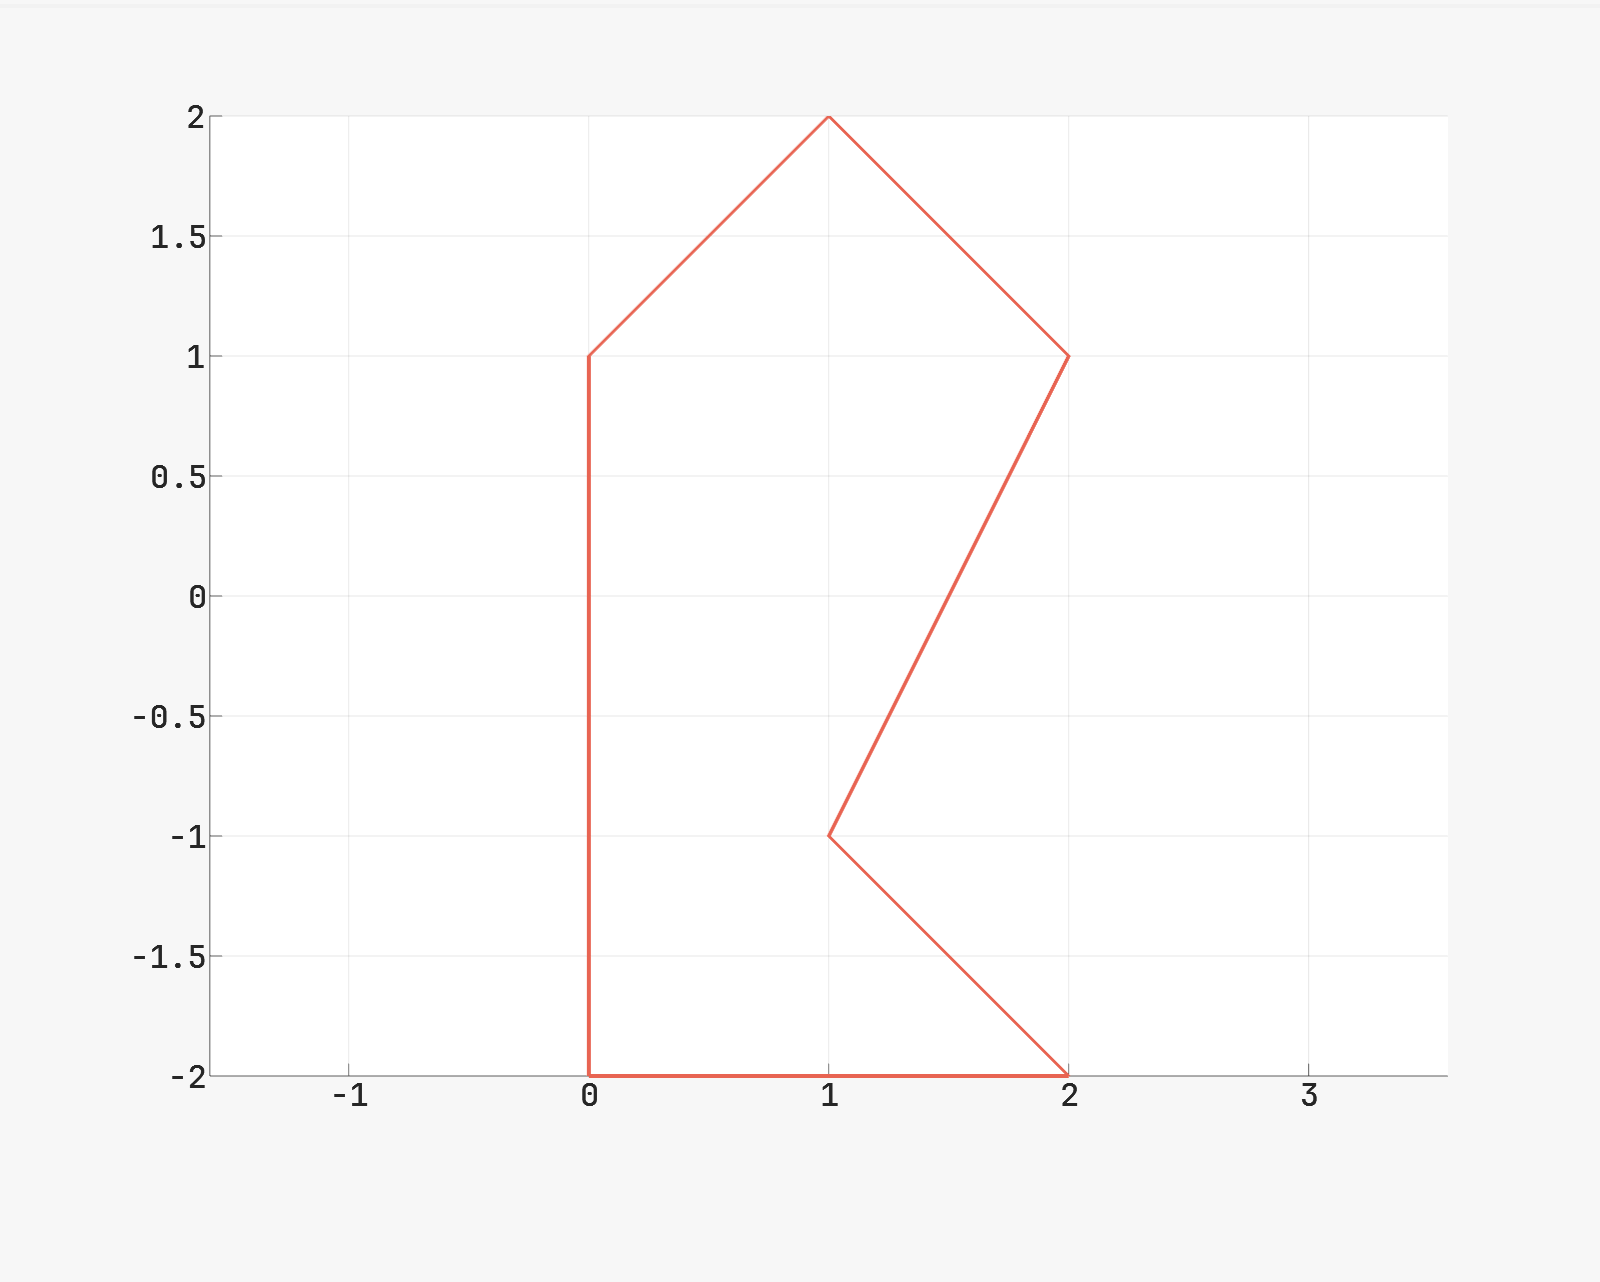
\includegraphics[width=0.9\linewidth]{Domain.png}
    \caption{Domain}
    \label{Domain}
\end{figure}
当$\alpha=0$得到Neumann边值问题,当$\beta=0$得到Dirichlet边值问题,所以我们设计该方程的对应有限差分格式,同时满足三类问题的求解。
\section{算法设计}
\subsection{网格离散}
在$x$和$y$方向以相同尺度$h$进行均匀剖分。令$n=1/h$,自下而上,从左至右,对Domain内的点及边界点进行编号,$0\leq i \leq 4n$,$0\leq j \leq j\_num[i]$。
所有点可分为三类:内点,边界点及临边界点,角点。
\subsection{算子离散及边界条件处理}
对于不同点进行不同格式离散:
\\ 对于内点,采取五点差分格式离散Laplace算子。
\\ 对于边界点,采取前向或者后向差商格式离散梯度,进而离散方向导数。
\\ 对于临边界点,即该点$(x,y)$非内点且不位于边界,则在边界上最近点为$(x^*,y^*)$,以点$(x,y)$的差商近似$(x^*,y^*)$的梯度,进而离散方向导数。
\\ 对于角点,赋予Dirichlet边界条件,即规定角点处取值为真实解。
\subsection{方程求解}
此线性方程组较为复杂,我们采取GMRES(m)迭代法进行求解。为了保证收敛性,先进行Gauss-Seidel迭代约100步,找到较为理想的初值,随后进行GMRES求解。
\section{数值结果}
\subsection{数值算例}
采取给定的数值算例,真实解$u(x,y)=\frac{\sin(\pi x)\cos(2\pi y)}{5\pi^2}$,进而源项$f(x,y)=\sin(\pi x)\cos(2\pi y)$。
\subsection{数值实验及结果}
对Dirichlet、Neumann、Robin三类边界条件均进行数值实验,所得结果位于文档ouput.txt,列表如\ref{数值结果展示}所示。
\begin{table}
    \centering
    \begin{tabular}{c c c c c}
        \hline
        边界条件&参数取值&$h$&GMRES迭代次数&$\|e_h\|_{\infty}$\\
        Dirichlet&alpha=1,beta=0&0.125&16&3.1e-3\\
        &&0.0625&48&1.6e-3\\
        &&0.03125&172&8.0e-4\\
        &&0.015625&619&4.0e-4\\
        &&0.0078125&2367&2.0e-4\\

        Neumann&alpha=0,beta=1&0.125&101&3.7e-2\\
        &&0.0625&502&1.9e-2\\
        &&0.03125&1169&9.7e-3\\
        &&0.015625&5983&5.0e-3\\
        &&0.0078125&31606&2.6e-3\\
        
        Robin&alpha=1,beta=1&0.125&42&1.7e-2\\
        &&0.0625&104&8.1e-3\\
        &&0.03125&321&4.0e-3\\
        &&0.015625&1831&2.0e-3\\
        &&0.0078125&8553&1.0e-3\\
        
    \end{tabular}
    \caption{数值结果展示}
    \label{数值结果展示}
\end{table}
\end{document}